\subsection{Intensidad de la onda}

La \textbf{intensidad de una onda} es una magnitud física que mide la energía transportada por unidad de tiempo y por unidad de área perpendicular a la dirección de propagación. En otras palabras, indica cuánta energía atraviesa una determinada superficie en un segundo debido al paso de una onda.

La intensidad \(I\) se define como:

\[
I = \frac{P}{S}
\]
donde:
\begin{itemize}
  \item \(P\) es la potencia transportada por la onda (energía por unidad de tiempo, en vatios),
  \item \(S\) es el área perpendicular a la dirección de propagación (en m²),
  \item \(I\) se expresa en vatios por metro cuadrado: \(\text{W/m}^2\).
\end{itemize}

Como la intensidad ``depende'' de la potencia, podemos deducir algunas características importantes. 

\paragraph{1. Proporcionalidad con la amplitud cuadrada}

La intensidad crece con el cuadrado de la amplitud de la onda (ya que la potencia es proporcional a la amplitud cuadrada):
\[
I \propto A^2
\]
Esto implica que una onda con el doble de amplitud transporta cuatro veces más energía por segundo y por área.

\paragraph{2. Disminución con la distancia}

En medios sin absorción, la intensidad de una onda esférica (como una onda sonora desde una fuente puntual) disminuye con el cuadrado de la distancia:
\[
I(r) = \frac{P}{4\pi r^2}
\]

Este resultado proviene del hecho de que la energía se distribuye sobre una superficie esférica que crece con \(r^2\), de ahí la ley del inverso del cuadrado.
\begin{figure}[ht]
  \centering
  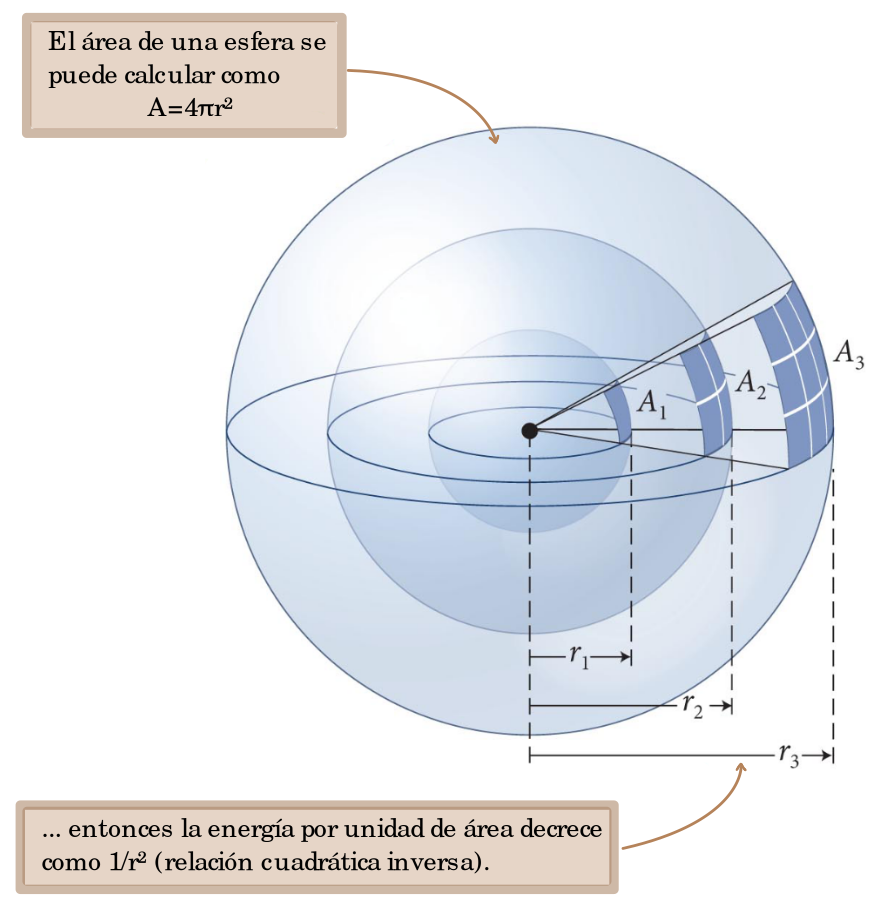
\includegraphics[width=0.6\textwidth]{intensity_decrease.png}
  \caption{Disminución de la intensidad con la distancia en una onda esférica.}
  \label{fig:intensity_decrease}
\end{figure}
Como se ve en la figura \ref{fig:intensity_decrease}, la potencia emitida es constante, sin embargo, a medida que el radio aumenta el área aumenta. Esto significa que la intensidad (es decir la potencia por uniad de área) es menor.

\paragraph{3. Medición directa de energía percibida}

En muchas aplicaciones físicas y técnicas (como en acústica o electromagnetismo), la intensidad está directamente relacionada con la sensación física percibida, como el volumen del sonido o la brillantez de la luz.

La intensidad de una onda cuantifica su capacidad de transportar energía a través del espacio. Es un parámetro fundamental cuando se estudian fenómenos como la absorción, reflexión, interferencia, o cuando se desea conocer el efecto físico de la onda en un sistema receptor.